\chapter{Os grupos funcionais e as famílias}\label{ch:g11:functional-groups}

Abra uma garrafa de vinagre, um frasco de removedor de esmalte, um
pacote de balas de pera, e passe por uma banca de peixe: quatro cheiros,
ácido, de \omterm{def:g6:solutions-and-solubility:solute}{solvente} adocicado, frutado e de peixe, e quatro tipos
diferentes de \omterm{def:g7:atoms-and-molecules:molecule}{molécula}. Cada uma deve o seu cheiro, e a maior parte da
sua química, não ao seu esqueleto de carbono, mas a um pequeno grupo de
\omterm{def:g7:atoms-and-molecules:atom}{átomos} ligado a ele: oxigênio e hidrogênio num caso, um \omterm{def:g7:atoms-and-molecules:atom}{átomo} de
nitrogênio em outro. Os químicos classificam os \omterm{def:g11:organic-skeletons:organic}{compostos orgânicos} por
esses grupos.

\begin{recall}
As \omterm{def:g11:organic-skeletons:formulas}{fórmulas em bastão}, os nomes dos \omterm{def:g11:organic-skeletons:alkane}{alcanos} e dos \omterm{def:g11:organic-skeletons:alkane}{grupos alquila}, os
\omterm{def:g11:organic-skeletons:isomer}{isômeros} (\cref{ch:g11:organic-skeletons}). As \omterm{def:g11:polarity-and-cohesion:polar-bond}{ligações polares} e as
\omterm{def:g11:polarity-and-cohesion:hydrogen-bond}{ligações de hidrogênio} (\cref{ch:g11:polarity-and-cohesion}).
\end{recall}

\begin{omfigure}
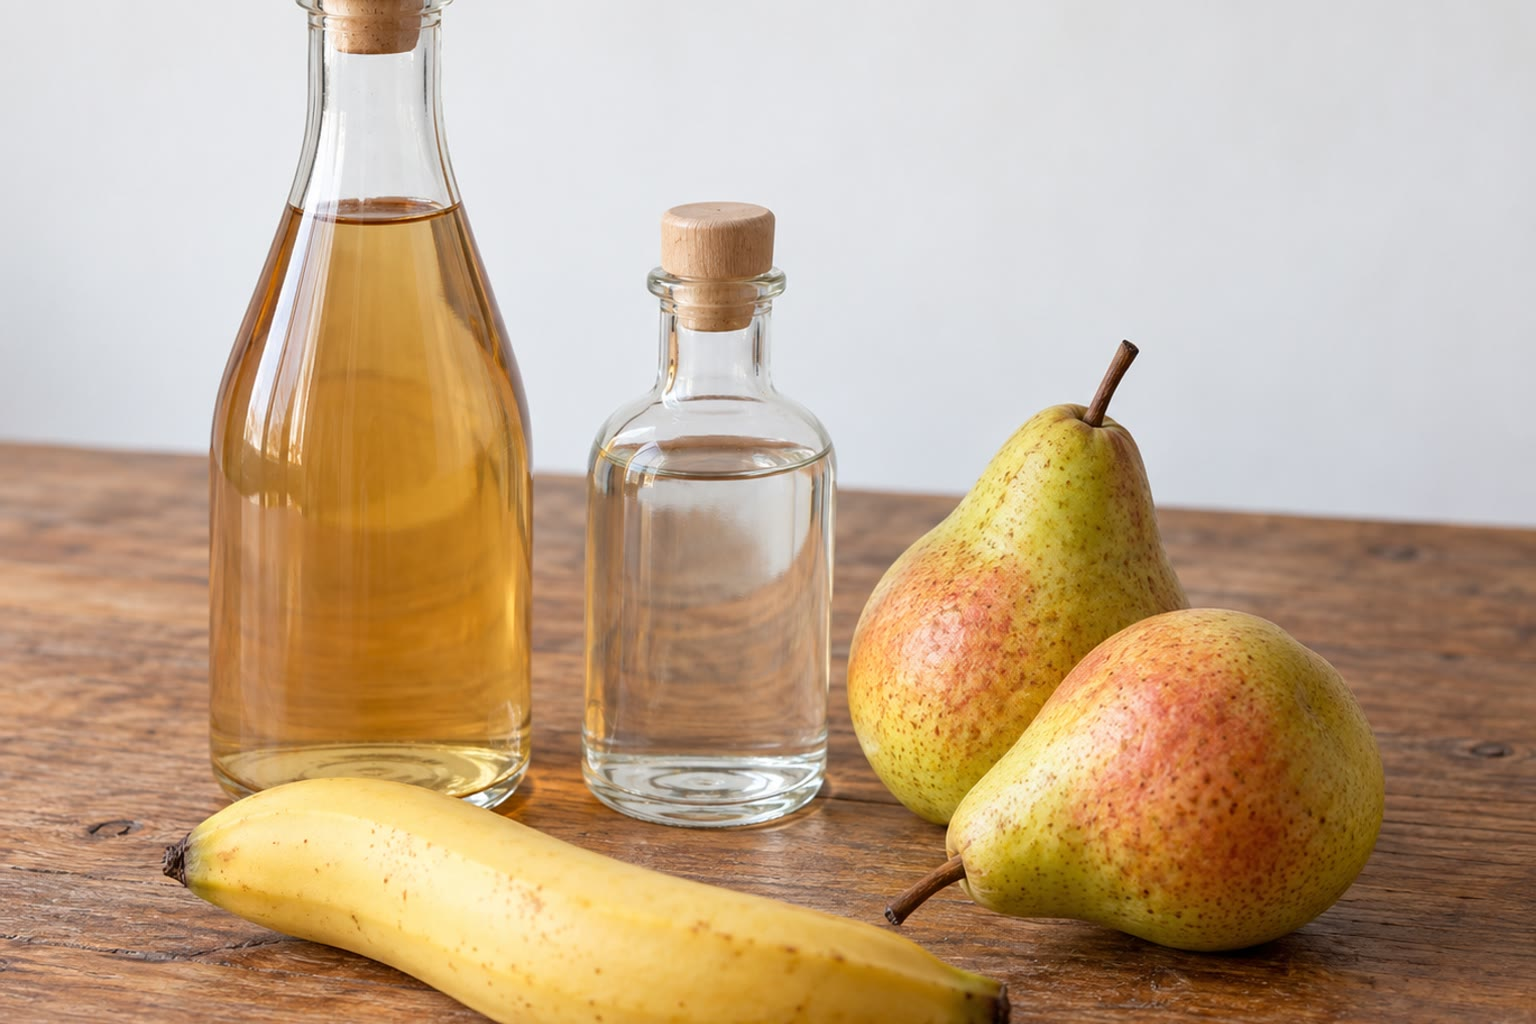
\includegraphics[width=0.5\linewidth]{images/book1/ai/g11-still-life-esters.jpg}

{\small Vinagre, um \omterm{def:g6:solutions-and-solubility:solute}{solvente}, frutas: cada cheiro vem de um grupo de
\omterm{def:g7:atoms-and-molecules:atom}{átomos} diferente num esqueleto de carbono.}
\end{omfigure}

\section{Os grupos funcionais}

\begin{definition}[Grupo funcional]\label{def:g11:functional-groups:functional-group}
Um \emph{grupo funcional}\index{grupo funcional} é um grupo de \omterm{def:g7:atoms-and-molecules:atom}{átomos},
além dos \omterm{def:g7:atoms-and-molecules:atom}{átomos} de carbono e de hidrogênio do esqueleto ligados só por
ligações simples, que dá a uma \omterm{def:g7:atoms-and-molecules:molecule}{molécula} as suas reações
características. Os compostos que compartilham um \omterm{def:g9:periodic-table-first-look:period}{grupo} funcional formam
uma família.
\end{definition}

\begin{omfigure}
\renewcommand{\arraystretch}{1.35}
\footnotesize
\begin{tabular}{@{}l@{\enspace}l@{\enspace}l@{\enspace}l@{\enspace}l@{}}
\hline
grupo & fórmula & família & terminação do nome & exemplo \\
\hline
hidroxila & \ce{-OH} & \omterm{def:g11:functional-groups:alcohol}{álcool} & \emph{-ol} & etanol, \ce{CH3-CH2-OH} \\
carbonila (na ponta) & \ce{-CHO} & \omterm{def:g11:functional-groups:carbonyl}{aldeído} & \emph{-al} & etanal, \ce{CH3-CHO} \\
carbonila (no meio) & \ce{C-CO-C} & \omterm{def:g11:functional-groups:carbonyl}{cetona} & \emph{-ona} & propanona, \ce{CH3-CO-CH3} \\
carboxila & \ce{-COOH} & \omterm{def:g11:functional-groups:carboxylic-acid}{ácido carboxílico} & \emph{ácido \ldots-oico} & ácido etanoico, \ce{CH3-COOH} \\
\omterm{def:g11:functional-groups:carboxylic-acid}{éster} & \ce{C-COO-C} & \omterm{def:g11:functional-groups:carboxylic-acid}{éster} & \emph{\ldots-oato de \ldots-ila} & etanoato de etila, \ce{CH3-COO-CH2-CH3} \\
\omterm{def:g11:functional-groups:amine}{amina} & \ce{-NH2} & \omterm{def:g11:functional-groups:amine}{amina} & \emph{-amina} & etanamina, \ce{CH3-CH2-NH2} \\
\omterm{def:g11:functional-groups:amine}{amida} & \ce{-CONH2} & \omterm{def:g11:functional-groups:amine}{amida} & \emph{-amida} & etanamida, \ce{CH3-CONH2} \\
\omterm{def:g10:electron-shells:family}{halogênio} & \ce{C-X} & \omterm{def:g11:functional-groups:halogenoalkane}{haloalcano} & prefixo \emph{cloro-}, \ldots & clorometano, \ce{CH3Cl} \\
\omterm{def:g10:lewis-and-shape:multiple-bond}{ligação dupla} & \ce{C=C} & \omterm{def:g11:functional-groups:halogenoalkane}{alceno} & \emph{-eno} & eteno, \ce{CH2=CH2} \\
\hline
\end{tabular}\par\medskip

\setchemfig{atom sep=1.4em}
\begin{tabular}{@{}c@{\quad}c@{\quad}c@{\quad}c@{\quad}c@{}}
\chemfig{R-C(=[2]O)-H} & \chemfig{R-C(=[2]O)-R'} & \chemfig{R-C(=[2]O)-O-H} &
\chemfig{R-C(=[2]O)-O-R'} & \chemfig{R-C(=[2]O)-N(-[1]H)-[7]H} \\
\small \omterm{def:g11:functional-groups:carbonyl}{aldeído} & \small \omterm{def:g11:functional-groups:carbonyl}{cetona} & \small \omterm{def:g11:functional-groups:carboxylic-acid}{ácido carboxílico} & \small \omterm{def:g11:functional-groups:carboxylic-acid}{éster} &
\small \omterm{def:g11:functional-groups:amine}{amida}
\end{tabular}\par\medskip

{\small Os principais \omterm{def:g11:functional-groups:functional-group}{grupos funcionais}, e os cinco construídos sobre um
grupo carbonila \ce{C=O}, desenhados por inteiro. R e R$'$ representam
cadeias de carbono (\omterm{def:g11:organic-skeletons:alkane}{grupos alquila}) e X um \omterm{def:g7:atoms-and-molecules:atom}{átomo} de \omterm{def:g10:electron-shells:family}{halogênio} (F, Cl, Br,
I).}
\end{omfigure}

\section{Os álcoois e a sua classe}

\begin{definition}[Álcool, classe de um álcool]\label{def:g11:functional-groups:alcohol}
Um \emph{álcool}\index{alcool@álcool} tem um grupo hidroxila \ce{-OH} ligado a
um \omterm{def:g7:atoms-and-molecules:atom}{átomo} de carbono que só tem ligações simples. A \emph{classe de um
álcool}\index{classe de um alcool@classe de um álcool} é primário, secundário ou terciário,
conforme o \omterm{def:g7:atoms-and-molecules:atom}{átomo} de carbono que leva o \ce{-OH} esteja ligado a um, a
dois ou a três outros \omterm{def:g7:atoms-and-molecules:atom}{átomos} de carbono. (O metanol, \ce{CH3OH}, cujo
carbono não está ligado a nenhum, é contado com os álcoois primários.)
\end{definition}

\begin{omfigure}
\setchemfig{atom sep=1.9em}
\begin{tabular}{ccc}
\chemfig{-[:30]-[:-30]-[:30]-[:-30]OH} &
\chemfig{-[:30](-[:90]OH)-[:-30]-[:30]} &
\chemfig{-[:0](-[:90]OH)(-[:-90])-[:0]} \\[4pt]
\small butan-1-ol & \small butan-2-ol & \small 2-metilpropan-2-ol \\
\small \textbf{primário} & \small \textbf{secundário} & \small \textbf{terciário} \\
\small (C do \ce{-OH}: 1 carbono vizinho) & \small (2 vizinhos) &
\small (3 vizinhos)
\end{tabular}

{\small Três \omterm{def:g11:organic-skeletons:isomer}{isômeros} \ce{C4H10O}, três classes de \omterm{def:g11:functional-groups:alcohol}{álcool}.}
\end{omfigure}

\section{Aldeídos, cetonas, ácidos e ésteres}

\begin{definition}[Aldeído, cetona]\label{def:g11:functional-groups:carbonyl}
Um grupo carbonila é uma \omterm{def:g10:lewis-and-shape:multiple-bond}{ligação dupla} \ce{C=O}. Se o seu \omterm{def:g7:atoms-and-molecules:atom}{átomo} de
carbono está na ponta da cadeia (ligado a pelo menos um \omterm{def:g7:atoms-and-molecules:atom}{átomo} de
hidrogênio), o composto é um \emph{aldeído}\index{aldeido@aldeído}; se ele está
no meio da cadeia (ligado a dois \omterm{def:g7:atoms-and-molecules:atom}{átomos} de carbono), o composto é uma
\emph{cetona}\index{cetona}.
\end{definition}

\begin{definition}[Ácido carboxílico, éster]\label{def:g11:functional-groups:carboxylic-acid}
Um \emph{ácido carboxílico}\index{acido carboxilico@ácido carboxílico} tem um grupo
carboxila \ce{-COOH}, uma carbonila e uma hidroxila no mesmo \omterm{def:g7:atoms-and-molecules:atom}{átomo} de
carbono. Um \emph{éster}\index{ester@éster} tem o grupo \ce{-COO-} entre duas
cadeias de carbono: ele é aparentado a um ácido cujo \ce{-OH} foi
substituído por um \ce{-O-}R$'$ vindo de um \omterm{def:g11:functional-groups:alcohol}{álcool}.
\end{definition}

\begin{example}[O etanoato de etila]\label{ex:g11:functional-groups:ethyl-ethanoate}
O \omterm{def:g6:solutions-and-solubility:solute}{solvente} etanoato de etila, \ce{CH3-COO-CH2-CH3}, tem cheiro de bala
de pera e de removedor de esmalte. A sua ``parte ácida'', \ce{CH3-CO},
vem do ácido etanoico \ce{CH3-COOH} e dá a primeira palavra do nome,
\emph{etanoato}; a sua ``parte alcoólica'', \ce{O-CH2-CH3}, vem do
etanol \ce{CH3-CH2-OH} e dá a segunda, \emph{de etila}. Um capítulo mais
adiante mostra como um \omterm{def:g11:functional-groups:carboxylic-acid}{éster} é produzido a partir do seu ácido e do seu
\omterm{def:g11:functional-groups:alcohol}{álcool}.
\end{example}

\begin{omfigure}
\setchemfig{atom sep=2.2em}
\chemfig{@{a}H_3C-@{c}C(=[2]@{o}O)-@{x}O-CH_2-@{z}CH_3}
\chemmove{
  \fill[omProp, opacity=0.14, rounded corners]
    ($(a.south west)+(-0.12,-0.15)$) rectangle ($(o.north east)+(0.25,0.12)$);
  \fill[omDef, opacity=0.14, rounded corners]
    ($(x.south west)+(-0.2,-0.15)$) rectangle ($(z.north east)+(0.4,0.75)$);
  \node[omProp, anchor=north east, align=right, font=\small] at ($(c.south)+(0.15,-0.25)$)
    {parte ácida, do ácido etanoico:\\ \emph{etanoato}};
  \node[omDef, anchor=north west, align=left, font=\small] at ($(x.south)+(0.05,-0.25)$)
    {parte alcoólica, do etanol:\\ \emph{de etila}};}
\par\vspace{1.4cm}

{\small Dar nome a um \omterm{def:g11:functional-groups:carboxylic-acid}{éster}: a parte ácida dá uma terminação em
\emph{-oato} (\emph{etanoato}), a parte alcoólica um nome de \omterm{def:g11:organic-skeletons:alkane}{grupo
alquila} (\emph{de etila}); o nome é ``etanoato de etila''.}
\end{omfigure}

\section{Aminas, amidas, haloalcanos e alcenos}


\begin{definition}[Amina, amida]\label{def:g11:functional-groups:amine}
Uma \emph{amina}\index{amina} tem um \omterm{def:g7:atoms-and-molecules:atom}{átomo} de nitrogênio ligado a uma
cadeia de carbono por uma ligação simples, como em \ce{-NH2}. Uma
\emph{amida}\index{amida} tem um \omterm{def:g7:atoms-and-molecules:atom}{átomo} de nitrogênio ligado ao carbono
de um grupo carbonila, como em \ce{-CO-NH2}.
\end{definition}

\begin{definition}[Haloalcano, alceno]\label{def:g11:functional-groups:halogenoalkane}
Um \emph{haloalcano}\index{haloalcano} é um \omterm{def:g11:organic-skeletons:alkane}{alcano} em que um ou mais
\omterm{def:g7:atoms-and-molecules:atom}{átomos} de hidrogênio foram substituídos por \omterm{def:g7:atoms-and-molecules:atom}{átomos} de \omterm{def:g10:electron-shells:family}{halogênio} (F, Cl,
Br, I). Um \emph{alceno}\index{alceno} tem uma \omterm{def:g10:lewis-and-shape:multiple-bond}{ligação dupla}
carbono--carbono, \ce{C=C}.
\end{definition}

\begin{remark}[Cheiros e grupos]\label{rem:g11:functional-groups:smells}
Muitas \omterm{def:g11:functional-groups:amine}{aminas} pequenas têm cheiro de peixe podre, e o cheiro do peixe
que já não está fresco se deve em grande parte a elas. Muitos \omterm{def:g11:functional-groups:carboxylic-acid}{ésteres}
pequenos têm cheiro de fruta. Os \omterm{def:g11:functional-groups:carboxylic-acid}{ácidos carboxílicos} pequenos têm um
cheiro ácido, como o vinagre; a propanona, uma \omterm{def:g11:functional-groups:carbonyl}{cetona}, é o conhecido
cheiro de \omterm{def:g6:solutions-and-solubility:solute}{solvente} do removedor de esmalte.
\end{remark}

\section{A nomenclatura}

\begin{method}[Dar nome a um composto orgânico com um grupo funcional]\label{met:g11:functional-groups:naming}
\begin{enumerate}
  \item Encontre a cadeia de carbono mais longa que \emph{contém} o
        carbono do \omterm{def:g11:functional-groups:functional-group}{grupo funcional} (ou, para um \omterm{def:g11:functional-groups:alcohol}{álcool} ou uma \omterm{def:g11:functional-groups:amine}{amina}, o
        carbono que o leva): ela dá o nome de base.
  \item Numere a cadeia a partir da extremidade que dá ao \omterm{def:g11:functional-groups:functional-group}{grupo funcional}
        o menor número.
  \item Troque o \emph{-o} do \omterm{def:g11:organic-skeletons:alkane}{alcano} pela terminação da família,
        precedida da posição do grupo se necessário: propan-2-ol,
        butan-2-ona. (Os \omterm{def:g11:functional-groups:carbonyl}{aldeídos}, os ácidos e as \omterm{def:g11:functional-groups:amine}{amidas} têm o seu grupo
        no carbono 1: sem número.)
  \item Acrescente os substituintes alquila como prefixos, com as suas
        posições, como nos \omterm{def:g11:organic-skeletons:alkane}{alcanos}; um \omterm{def:g10:electron-shells:family}{halogênio} é sempre um prefixo
        (2-cloropropano).
\end{enumerate}
\end{method}

\begin{example}[Quatro nomes]\label{ex:g11:functional-groups:names}
\setchemfig{atom sep=1.7em}
\chemfig{-[:30](-[:90]OH)-[:-30]} é o propan-2-ol (um \omterm{def:g11:functional-groups:alcohol}{álcool} secundário);
\chemfig{-[:30](=[:90]O)-[:-30]-[:30]} é a butan-2-ona;
\chemfig{-[:30]-[:-30]-[:30](=[:90]O)-[:-30]OH} é o ácido butanoico;
\chemfig{-[:30](-[:90])-[:-30]-[:30]=[:-30]O} é o 3-metilbutanal.
\end{example}

\begin{omfigure}
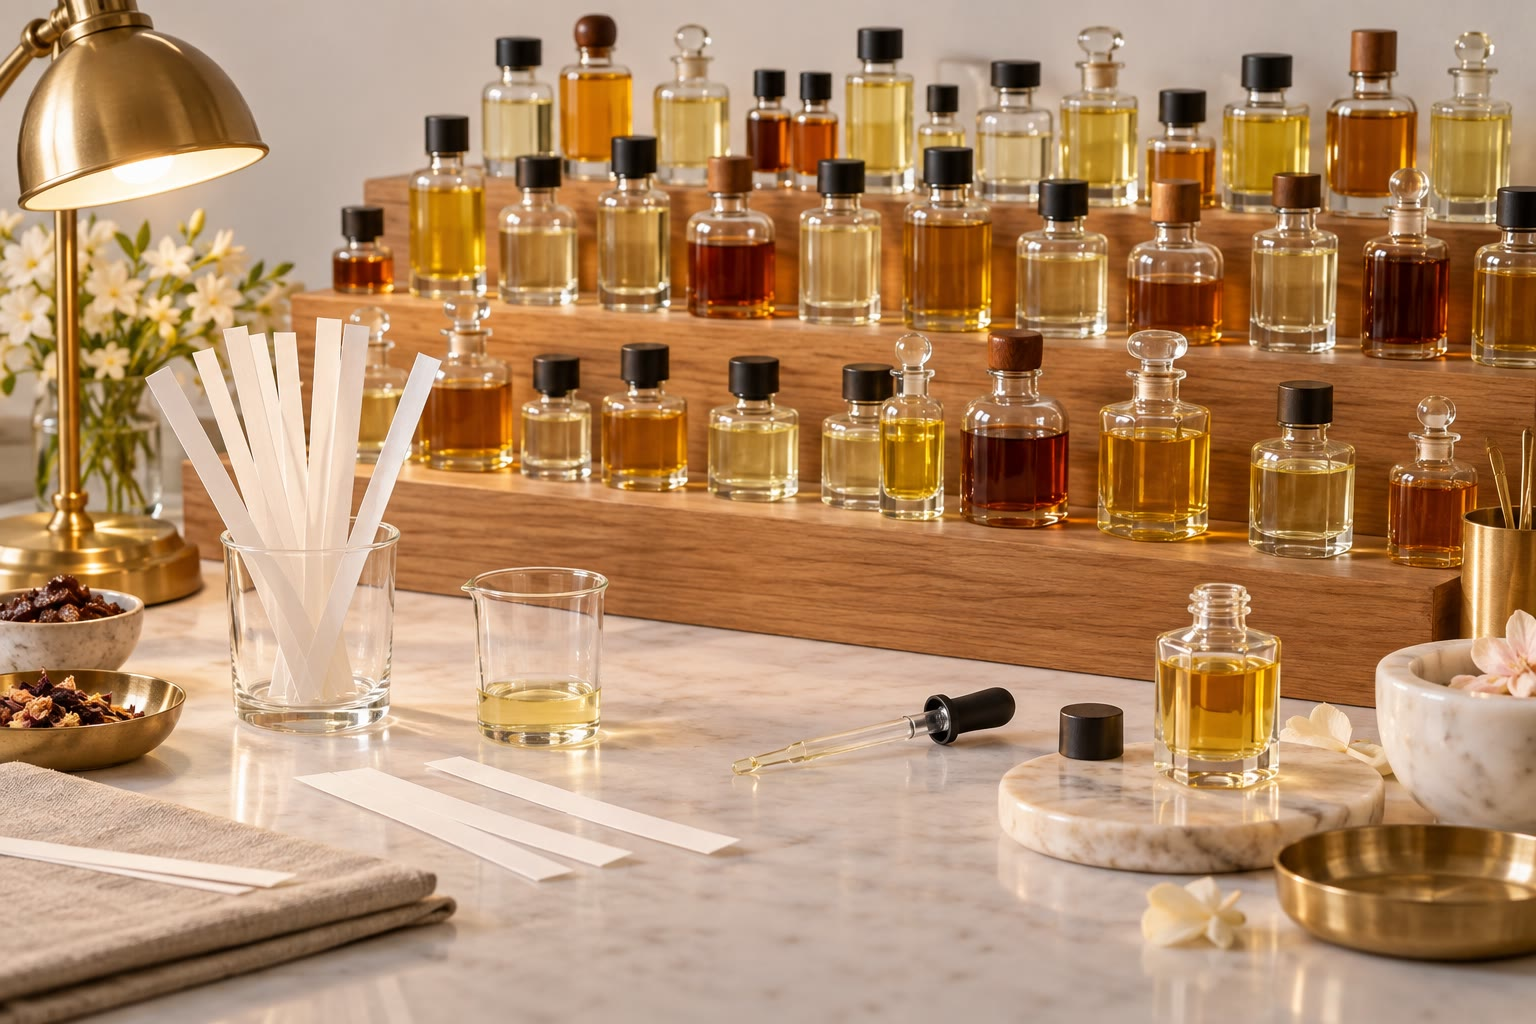
\includegraphics[width=0.48\linewidth]{images/book1/ai/g11-perfumer-lab.jpg}

{\small A bancada de um perfumista: muitos dos frascos contêm \omterm{def:g11:functional-groups:carboxylic-acid}{ésteres},
\omterm{def:g11:functional-groups:alcohol}{álcoois}, \omterm{def:g11:functional-groups:carbonyl}{aldeídos} e \omterm{def:g11:functional-groups:carbonyl}{cetonas}.}
\end{omfigure}

\begin{safety}{\ghs[0.82cm]{GHS02}\ghs[0.82cm]{GHS05}\ghs[0.82cm]{GHS07}}
% ledger: ghs:acetone, ghs:acetic-acid
A propanona é altamente inflamável e irritante para os olhos; o seu
vapor dá sonolência. O ácido etanoico puro é inflamável e provoca
queimaduras graves na pele e nos olhos; o vinagre é uma solução diluída
dele. Os cheiros nunca são testados cheirando um frasco: o vapor é
abanado devagar em direção ao nariz com a mão, e só quando o professor
autoriza.
\end{safety}

\section{Exercícios}


\begin{exercise}[$\star$]\label{exo:g11:functional-groups:1}
Dê o nome do \omterm{def:g11:functional-groups:functional-group}{grupo funcional} e da família de cada composto:
\ce{CH3-CH2-CH2-OH}; \ce{CH3-CO-CH2-CH3}; \ce{CH3-CH2-COOH};
\ce{CH3-COO-CH3}; \ce{CH3-CH2-NH2}.
\end{exercise}

\begin{exercise}[$\star$]\label{exo:g11:functional-groups:2}
Dê o nome: \ce{CH3-OH}; \ce{CH3-CH2-CH2-OH}; \ce{HCOOH}; \ce{CH3-CH2-CHO};
\ce{CH3-CO-CH3}.
\end{exercise}

\begin{exercise}[$\star$]\label{exo:g11:functional-groups:3}
A que família pertence cada composto: butan-2-ol, pentanal, propanoato
de metila, propanamida, 2-bromopropano, but-1-eno?
\end{exercise}

\begin{exercise}[$\star$]\label{exo:g11:functional-groups:4}
Escreva as \omterm{def:g11:organic-skeletons:formulas}{fórmulas estruturais condensadas} do propanal e da propanona.
Qual é o \omterm{def:g11:functional-groups:carbonyl}{aldeído}? Como se reconhece?
\end{exercise}

\begin{exercise}[$\star$]\label{exo:g11:functional-groups:5}
Dê a classe do propan-1-ol, do propan-2-ol e do 2-metilpropan-2-ol.
\end{exercise}

\begin{exercise}[$\star\star$]\label{exo:g11:functional-groups:6}
Desenhe as \omterm{def:g11:organic-skeletons:formulas}{fórmulas em bastão} do pentan-3-ol, do ácido
2-metilbutanoico, da hexan-2-ona e do etanoato de propila.
\end{exercise}

\begin{exercise}[$\star\star$]\label{exo:g11:functional-groups:7}
O propanal e a propanona têm a mesma \omterm{def:g11:organic-skeletons:formulas}{fórmula molecular}. Dê-a. Eles são
\omterm{def:g11:organic-skeletons:isomer}{isômeros}? Eles têm o mesmo \omterm{def:g11:functional-groups:functional-group}{grupo funcional}?
\end{exercise}

\begin{exercise}[$\star\star$]\label{exo:g11:functional-groups:8}
Escreva a \omterm{def:g11:organic-skeletons:formulas}{fórmula estrutural condensada} e o nome do \omterm{def:g11:functional-groups:carboxylic-acid}{éster} cuja parte
ácida vem do ácido metanoico \ce{HCOOH} e cuja parte alcoólica vem do
etanol; depois, do \omterm{def:g11:functional-groups:carboxylic-acid}{éster} do ácido etanoico e do propan-1-ol.
\end{exercise}

\begin{exercise}[$\star\star$]\label{exo:g11:functional-groups:9}
Dê o nome dos \omterm{def:g11:functional-groups:carboxylic-acid}{ésteres} \ce{CH3-COO-CH3}, \ce{CH3-CH2-COO-CH2-CH3} e
\ce{HCOO-CH3}, e o ácido e o \omterm{def:g11:functional-groups:alcohol}{álcool} a que cada um é aparentado.
\end{exercise}

\begin{exercise}[$\star\star$]\label{exo:g11:functional-groups:10}
Desenhe e dê o nome dos quatro \omterm{def:g11:functional-groups:alcohol}{álcoois} de fórmula \ce{C4H10O}, e dê a
classe de cada um.
\end{exercise}

\begin{exercise}[$\star\star$]\label{exo:g11:functional-groups:11}
Usando a tabela dos grupos: qual é a família de \ce{CH3-CO-NH2}? Que
terminação o nome de um \omterm{def:g11:functional-groups:halogenoalkane}{alceno} recebe? Que famílias têm um grupo
carbonila com um \omterm{def:g7:atoms-and-molecules:atom}{átomo} de oxigênio ou de nitrogênio no mesmo carbono?
\end{exercise}

\begin{exercise}[$\star\star\star$]\label{exo:g11:functional-groups:12}
Circule e dê o nome dos \omterm{def:g11:functional-groups:functional-group}{grupos funcionais} da aspirina e do paracetamol.
(Um \ce{-OH} ligado diretamente a um anel como o do paracetamol se chama
grupo fenol; ele se comporta de modo diferente de um \omterm{def:g11:functional-groups:alcohol}{álcool}.)
\begin{center}
\setchemfig{atom sep=1.6em}
\chemfig{*6(-=-(-COOH)=(-O-[:150]C(=[:90]O)-[:210]H_3C)-=)}
\qquad
\chemfig{*6((-OH)=-=(-N(-[2]H)-[7]C(=[6]O)-[1]CH_3)-=-)}
\\[2pt] \small aspirina \hspace{4.2cm} paracetamol
\end{center}
\end{exercise}

\begin{exercise}[$\star\star\star$]\label{exo:g11:functional-groups:13}
% ledger: bp:C2H5OH, bp:CH3OCH3
O etanol \ce{CH3-CH2-OH} e o metoximetano \ce{CH3-O-CH3} têm a mesma
\omterm{def:g11:organic-skeletons:formulas}{fórmula molecular}. Dê-a. O metoximetano pertence a uma família que não
está na tabela, a dos éteres. Qual dos dois pode formar \omterm{def:g11:polarity-and-cohesion:hydrogen-bond}{ligações de
hidrogênio} entre as suas próprias \omterm{def:g7:atoms-and-molecules:molecule}{moléculas}? Qual ferve a uma
temperatura mais alta (um ferve a \qty{78}{\celsius}, o outro a
\qty{-25}{\celsius})?
\end{exercise}

\begin{exercise}[$\star\star\star$]\label{exo:g11:functional-groups:14}
O ácido lático, produzido pelos músculos cansados, é
\chemfig{CH_3-CH(-[2]OH)-COOH}. Dê o nome dos seus dois \omterm{def:g11:functional-groups:functional-group}{grupos
funcionais}. Quando uma \omterm{def:g7:atoms-and-molecules:molecule}{molécula} tem um grupo ácido e outro grupo, o
ácido dá a terminação e o outro grupo vira um prefixo (\emph{hidroxi-}
para \ce{-OH}, \emph{amino-} para \ce{-NH2}). Dê o nome do ácido lático,
e depois o da glicina, \ce{H2N-CH2-COOH}.
\end{exercise}

\begin{exercise}[$\star\star\star$]\label{exo:g11:functional-groups:15}
O vinho deixado aberto ao \omterm{def:g4:air-a-mixture-of-gases:air}{ar} vira vinagre: o etanol vira ácido etanoico,
passando pelo etanal. Escreva as \omterm{def:g11:organic-skeletons:formulas}{fórmulas estruturais condensadas} e
moleculares dos três compostos e as suas famílias. O que muda na
fórmula em cada etapa?
\end{exercise}

\section{Problema: os aromas de fruta}

\begin{problem}[{Problema de fim de semana --- uma química de aromas
constrói o cheiro de banana: qual é a massa molar da molécula-chave?}]
\label{pb:g11:functional-groups:1}
% ledger: aw:C, aw:H, aw:O
Uma química de aromas tem cinco compostos na sua bancada:
\begin{center}
\begin{tabular}{ll}
A & \chemfig{CH_3-C(=[2]O)-O-CH_2-CH_2-CH(-[2]CH_3)-CH_3} \\[16pt]
B & \chemfig{HO-CH_2-CH_2-CH(-[2]CH_3)-CH_3} \\[10pt]
C & \ce{CH3-COOH} \\
D & \ce{CH3-CH2-CH2-CH2-CH2-CHO} \\
E & \ce{CH3-CH2-CH2-COO-CH2-CH3}
\end{tabular}
\end{center}
A tem cheiro de banana e de bala de pera, B de malte, C de vinagre, D
de grama cortada, E de abacaxi.

\medskip
\noindent\textbf{Parte I --- Grupos e famílias.}
\begin{enumerate}
  \item Dê o nome do \omterm{def:g11:functional-groups:functional-group}{grupo funcional} de cada composto.
  \item Dê a família de cada um.
  \item Que compostos são \omterm{def:g11:functional-groups:carboxylic-acid}{ésteres}? Que cheiros eles têm?
  \item Qual é a classe do \omterm{def:g11:functional-groups:alcohol}{álcool} B?
  \item Dê a \omterm{def:g11:organic-skeletons:formulas}{fórmula molecular} de D, e desenhe um \omterm{def:g11:organic-skeletons:isomer}{isômero} de D que seja
        uma \omterm{def:g11:functional-groups:carbonyl}{cetona}.
\end{enumerate}

\medskip
\noindent\textbf{Parte II --- Os nomes.}
\begin{enumerate}[resume]
  \item Dê o nome de B (encontre a cadeia mais longa que contém o
        carbono que leva o \ce{-OH}).
  \item Dê o nome de C e de D.
  \item Dê o nome de E, e o ácido e o \omterm{def:g11:functional-groups:alcohol}{álcool} a que ele é aparentado.
  \item Explique o nome de A, etanoato de 3-metilbutila: que parte vem
        do ácido, e que parte vem do \omterm{def:g11:functional-groups:alcohol}{álcool}?
\end{enumerate}

\medskip
\noindent\textbf{Parte III --- A partir de um ácido e de um \omterm{def:g11:functional-groups:alcohol}{álcool}.}
\begin{enumerate}[resume]
  \item A que dois compostos da bancada A é aparentado?
  \item Dê as \omterm{def:g11:organic-skeletons:formulas}{fórmulas moleculares} de A, B e C.
  \item Um \omterm{def:g11:functional-groups:carboxylic-acid}{éster} é produzido a partir do seu ácido e do seu \omterm{def:g11:functional-groups:alcohol}{álcool}, com
        perda de uma pequena \omterm{def:g7:atoms-and-molecules:molecule}{molécula}. Usando as fórmulas, descubra qual.
  \item Escreva a equação da formação de A, em \omterm{def:g11:organic-skeletons:formulas}{fórmulas moleculares}, e
        verifique que ela está balanceada.
\end{enumerate}

\medskip
\noindent\textbf{Parte IV --- \omterm{def:g10:the-mole:molar-mass}{Massas molares}.}
\begin{enumerate}[resume]
  \item Calcule as \omterm{def:g10:the-mole:molar-mass}{massas molares} de B e de C.
  \item Deduza a \omterm{def:g10:the-mole:molar-mass}{massa molar} de A a partir da equação da questão 13.
  \item Calcule a \omterm{def:g10:the-mole:molar-mass}{massa molar} de A diretamente a partir da sua fórmula,
        e compare.
  \item Verifica-se que uma amostra frutada desconhecida tem \omterm{def:g10:the-mole:molar-mass}{massa molar}
        próxima de \qty{116}{g/mol}. Ela é A ou E?
  \item O ácido heptanoico, \ce{CH3-(CH2)5-COOH}, tem cheiro de ranço.
        Mostre que ele é um \omterm{def:g11:organic-skeletons:isomer}{isômero} de A. Uma \omterm{def:g10:the-mole:molar-mass}{massa molar} sozinha
        consegue identificar um composto?
  \item Por que os químicos dizem que o cheiro pertence ao \omterm{def:g11:functional-groups:functional-group}{grupo
        funcional} tanto quanto ao esqueleto? Use A e o ácido heptanoico.
  \item Dê a resposta final: qual é a \omterm{def:g10:the-mole:molar-mass}{massa molar} do \omterm{def:g11:functional-groups:carboxylic-acid}{éster} da banana, o
        etanoato de 3-metilbutila?
\end{enumerate}
\end{problem}
